 \chapter{Risultati} \label{chap:risultati}

% **************************** Define Graphics Path **************************
\ifpdf
    \graphicspath{{Chapter7/Figs/Raster/}{Chapter7/Figs/PDF/}{Chapter7/Figs/}}
\else
    \graphicspath{{Chapter7/Figs/Vector/}{Chapter7/Figs/}}
\fi



\section{Istanze e risultati}
Abbiamo preso in considerazione due tipologie di istanze, basate sui set di posizioni $P$ e illustrate in \figurename\ \ref{figP}, rappresentanti diversi scenari. 
Different instances have been considered based on the sets $P$ depicted in Figure , representing different deployment scenarios.
%
\begin{figure}
	\begin{center}
		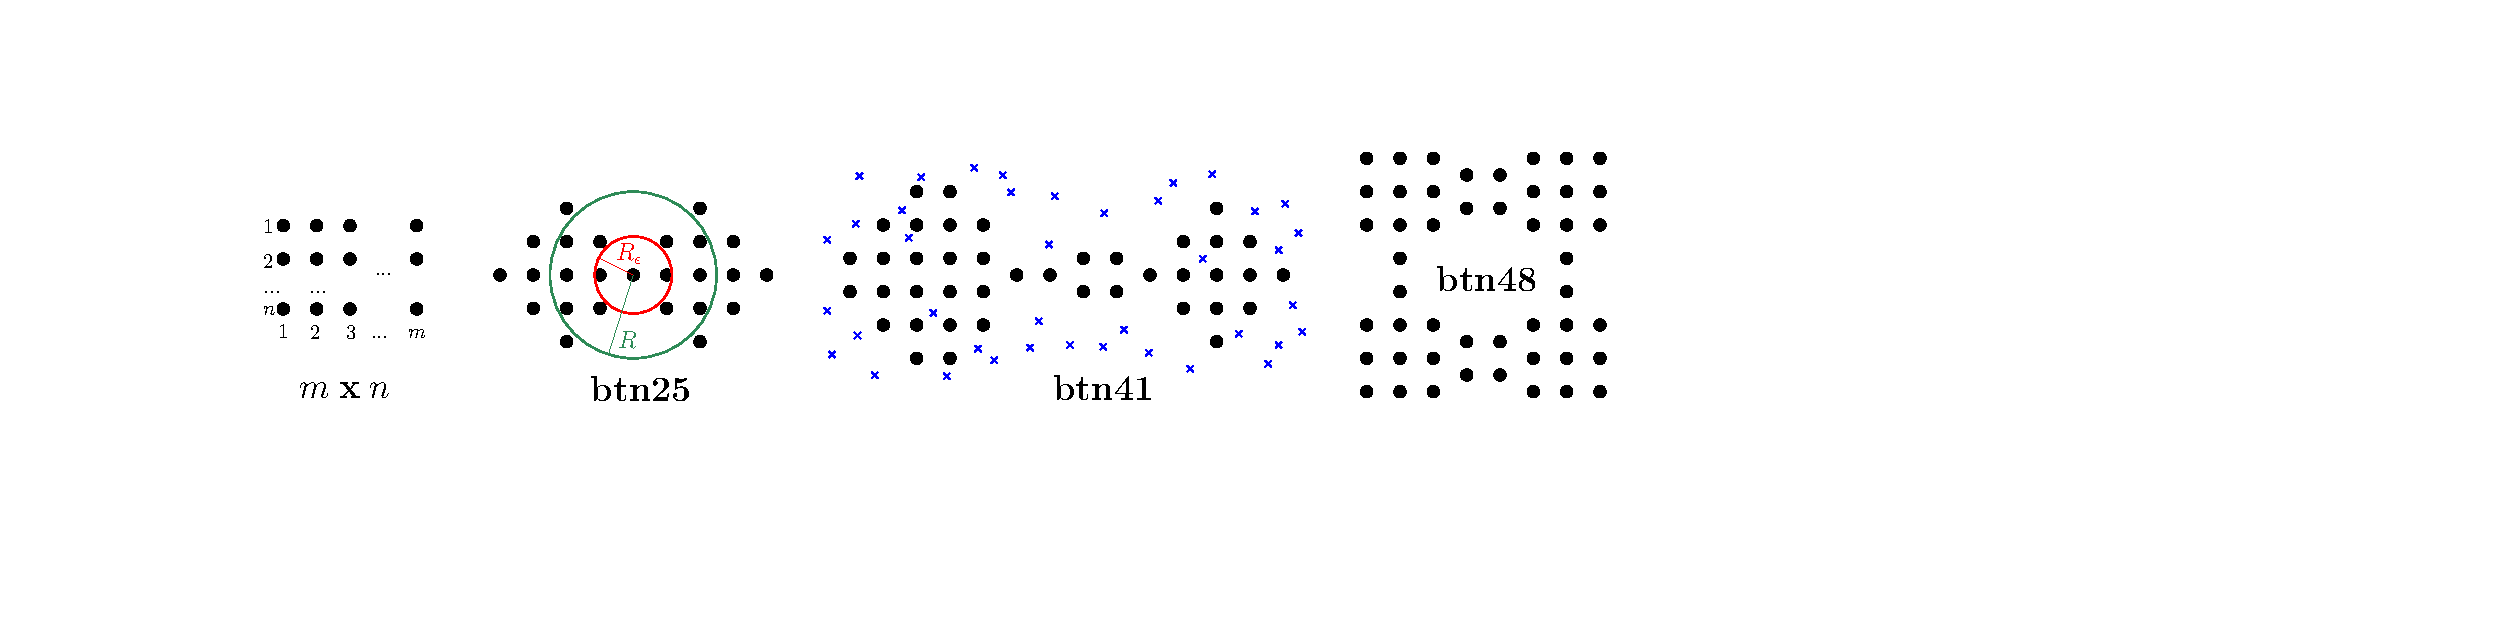
\includegraphics[scale=0.60]{figTopolHorUsersP}
	\end{center}
	\caption{Tipologie di griglie utilizzate.} \label{figP}
\end{figure}
%
Le posizioni degli utenti sono state generate in maniera casuale attorno all'area della griglia, assicurandosi che tutti i client si trovassero a distanze minori di $R$ da ciascun punto $i \in P$, per evitare istanze impossibili da risolvere a causa del cattivo posizionamento. 
Users' positions have been generated at random in the area including all the points at distance $R$ from any $i \in P$, with clients more likely to be close to the borders (e.g. the blue crosses in Figure \ref{figP}). For each set and each number of users in the set $\{20,40,60,80,100\}$, 3 instances have been generated, using homogeneous node settings. \ref{tabRes}.
%

Come detto nel \chaptername\ \ref{cap:metodi}, il modello è stato implementato in C++ utilizzando le CPLEX Callable Library (C API), con tempo massimo di esecuzione di 40 minuti, parallelismo deterministico e focus sull'ottimizzazione della memoria.Le istanze sono state risolte su un sistema con 4 processori Intel Xeon E5520 @2.27 GHz e 32 GB di RAM. \\

\setlength{\tabcolsep}{3.5 pt}
\renewcommand\arraystretch{1.1}
\begin{table} 
	\scriptsize
	\center
	\begin{tabular}{lc|rrrr|rrr|rrr}
		\hline
		\multicolumn{2}{c}{\bf Instance} & \multicolumn{4}{|c}{{\bf Cplex 12.6}} & \multicolumn{3}{|c}{{\bf Heur. 1}} & \multicolumn{3}{|c}{{\bf Heur. 2}}\\
		{\bf $P$} & $|V|$ & LP gap & Best & Time & win & Best & Time & win & Best & Time & win \\
		\hline
		9x3 & 20 & 1 & 2 & 3 & 4 & 1 & 2 & 3 & 1 & 2 & 3 \\
		9x3 & 40 & 1 & 2 & 3 & 4 & 1 & 2 & 3 & 1 & 2 & 3 \\
		btn25 & 30 & 1 & 2 & 3 & 4 & 1 & 2 & 3 & 1 & 2 & 3 \\
		7x7 & 40 & 1 & 2 & 3 & 4 & 1 & 2 & 3 & 1 & 2 & 3 \\
		12x4 & 40 & 1 & 2 & 3 & 4 & 1 & 2 & 3 & 1 & 2 & 3 \\
		btn41 & 30 & 1 & 2 & 3 & 4 & 1 & 2 & 3 & 1 & 2 & 3 \\
		btn41 & 50 & 1 & 2 & 3 & 4 & 1 & 2 & 3 & 1 & 2 & 3 \\
		btn41 & 70 & 1 & 2 & 3 & 4 & 1 & 2 & 3 & 1 & 2 & 3 \\
		btn48 & 30 & 1 & 2 & 3 & 4 & 1 & 2 & 3 & 1 & 2 & 3 \\
		btn48 & 50 & 1 & 2 & 3 & 4 & 1 & 2 & 3 & 1 & 2 & 3 \\
		btn48 & 70 & 1 & 2 & 3 & 4 & 1 & 2 & 3 & 1 & 2 & 3 \\
		8x8 & 30 & 1 & 2 & 3 & 4 & 1 & 2 & 3 & 1 & 2 & 3 \\
		10x10 & 30 & 1 & 2 & 3 & 4 & 1 & 2 & 3 & 1 & 2 & 3 \\
		10x10 & 50 & 1 & 2 & 3 & 4 & 1 & 2 & 3 & 1 & 2 & 3 \\
		\hline
	\end{tabular}
	\normalsize
	\caption{Experimental results.} 
	\label{tabRes}
\end{table}
%